\chapter{Iteracion 7: Caso de prueba con un sensor de campo electrostatico} % (fold)
\label{cha:iteracion_7}

\section{Introduccion} % (fold)
\label{sec:introduccion}

Parte de este proyecto fue poner a prueba nuestro sistema utilizando un sensor detector de campo electrostatico. Ademas de obtener las mediciones, fue necesario realizar un sistema de control para el motor del sensor. En esta iteracion realizamos la adaptacion necesaria de los requisitos de funcionamiento del sensor a nuestro sistema de instrumentacion, probando asi el funcionamiento del mismo, asi como tambien el funcionamiento del sistema gestionador desarrollado en la iteracion \ref{cha:iteracion_6} 

\subsection{Marco teorico} % (fold)
\label{sub:marco_teorico}

La intensidad de un campo electrico se puede medir, en principio, colcando un medidor de voltaje entre dos placas metalicas paralelas separadas por una distancia. El problema de esto es que, como el medidor de voltaje suele tener una impedancia alta en la entrada, cualquier voltaje inducido en las placas se pierde rapidamente, y no podria usarse para medir el capo electrico. Para arreglar esto, se utiliza la tecnica de las aspas. Se coloca una placa conductora, y sobre la misma se posiciona un sistema con aspas de forma que cuando estas roten, se cubra y se exponga periodicamente la placa conductora al campo electrico ambiental. Para lograr esto apropiadamente, el rotor que hace girar las aspas debe estar conectado a tierra. La placa conductora esta conectada a tierra a traves de un amplificador de transconductancia, que convierte la corriente que va desde la placa a tierra en una tension.
A medida que la placa conductora este expuesta al campo electrico, el campo induce una corriente a tierra mientras que atrae o repele la carga de la placa conductora. A medida que la placa esta cubierta del campo electrico, la carga inducida se drena. Entonces las placas inducen una corriente alterna a masa que es proporcional a la intensidad del campo electrico estatico. Esta corriente alterna luego puede ser rectificada para utilizarla como entrada a un conversor analogico digital y obtener asi la intensidad del campo electrico medido. \\

Una vez obtenida la intensidad, es necesario saber el signo del campo electrico medido. Para obtenerlo, un metodo es que en el mismo conversor analogico digital se obtenga la medicion de manera diferencial. Un conversor analogico digital diferencial toma la diferencia entre dos canales para obtener un dato en lugar de tomar el valor de un canal y compararlo con tierra. De forma que es posible determinar cual es el canal con mayor tension. Con esto, se pueden conectar los canales de las señales de tierra y la de la placa conductora, y se miden de manera diferencial para obtener tento la intensidad como el signo del campo electrico estatico.
\cite{sensorcampo}

% subsection marco_teorico (end)
\subsection{El sensor} % (fold)
\label{sub:el_sensor}

El sensor utilizado es un dispositivo que mide la intensidad del campo electrico en el ambiente debido al campo electrostatico generado por la carga electrica de las nubes en el momento. Se puede utilizar para detectar la posibilidad de que caiga un rayo en una zona cercana al sensor, y tambien para investigar los efectos de la electricidad estatica. Para funcionar, el sensor necesita de un motor que gire a velocidad constante. Este motor funciona en base a un driver que tiene como entrada una señal modulada por ancho de pulso.
Mientras el motor gire a velocidad constante, es posible obtener datos validos del sensor. La idea es hacer que el funcionamiento del sensor como la adquisicion de las mediciones sea logrado con funcionalidades de la placa de instrumentacion, mas otras caracteristicas que ofrece el microcontrolador C8051F352, como ser el modulo de PWM para generar la señal modulada por ancho de pulso, y el uso de los timers para establecer las bases de tiempo que utilizamos para hacer un control de estabilidad en la velocidad del motor. \\

Fisicamente, es una estructura metalica compuesta por un motor que hace girar unas aspas que se se encargan de blindar y desblindar una placa que a su vez se carga y descarga con la electricidad estatica del ambiente. esta carga y descarga continua es lo que justamente se termina transformando en el nivel de voltaje que nos indica el nivel de electricidad estatica del ambiente, que es lo que queremos saber.
La placa y las aspas funcionan como un capacitor que se blinda y se des\-blinda a medida que el motor gira. En el momento que las aspas estan descuburiendo la placa, el capacitor se carga, y en el momento que se cubre la placa, el capacitor se descarga. La descarga se hace sobre un amplificador que luego va a un conversor analogico digital, que termina en la lectura de un valor que nos dice el nivel del campo electrostatico ambiental. En el caso particular de este sensor, el motor que hace girar las aspas es un motor brushless manejado por un driver PWM.

\begin{figure}[h]
  \centering
  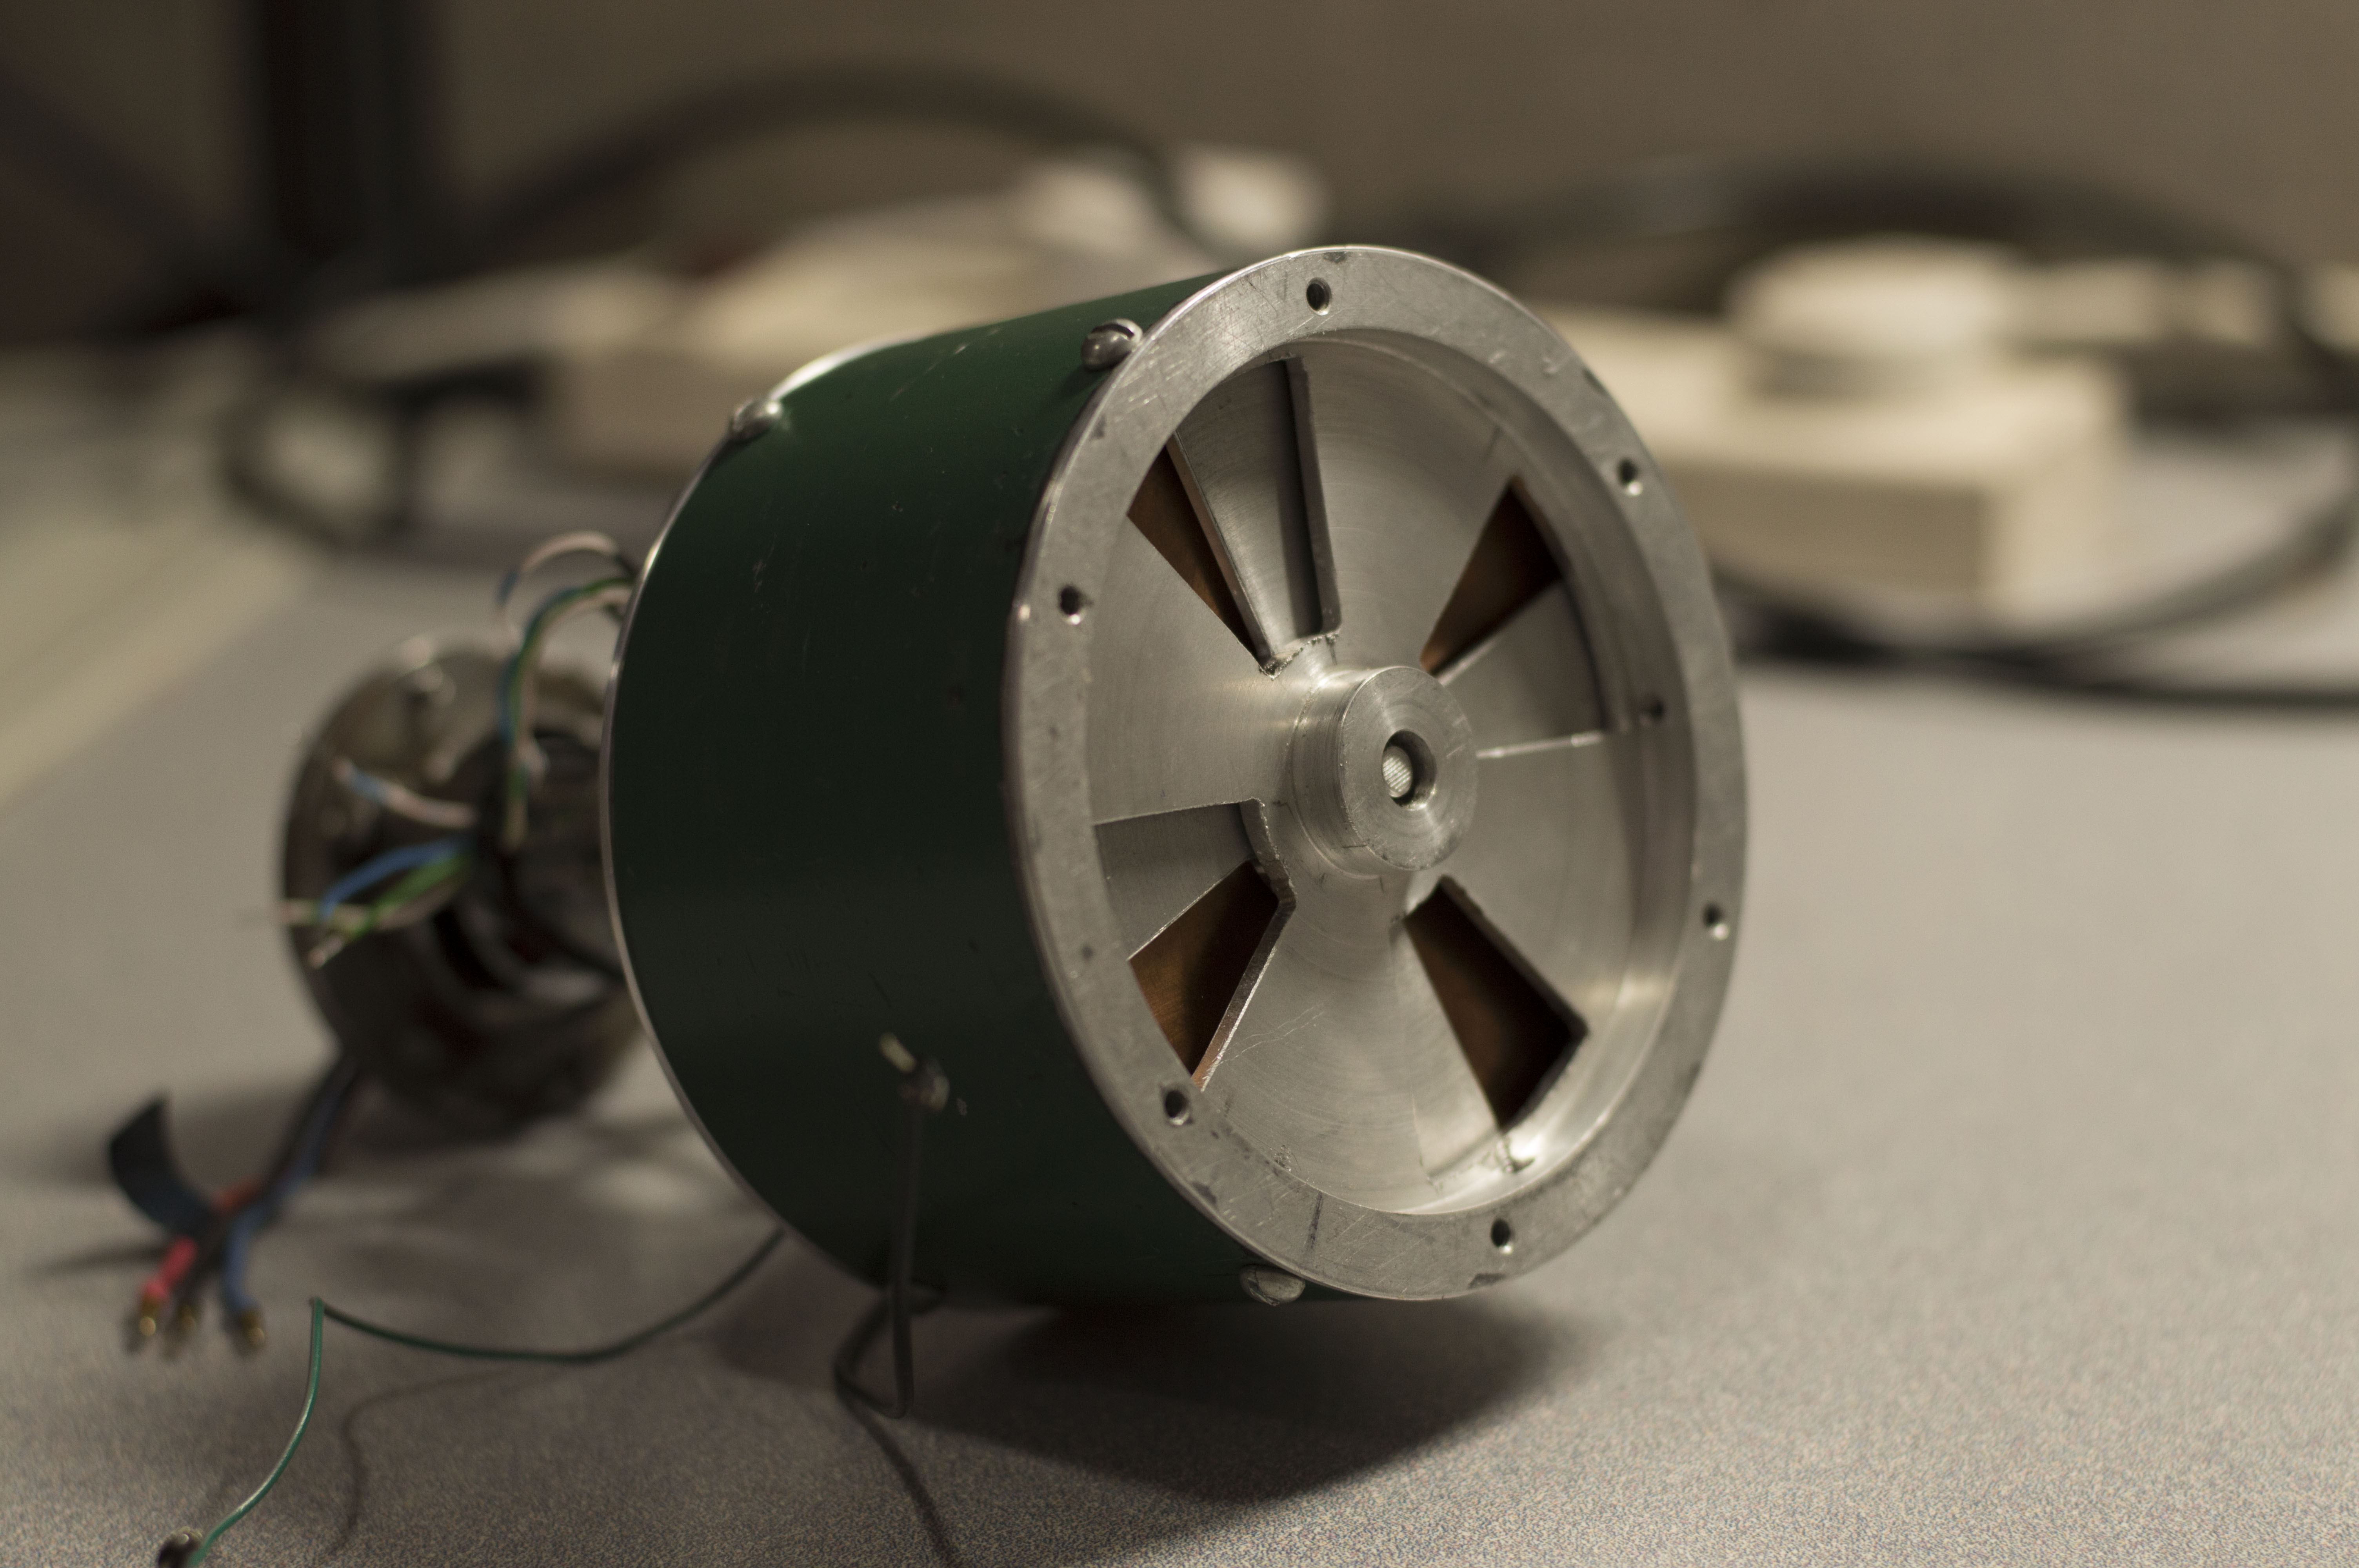
\includegraphics[width=0.80\textwidth, height = 7cm]{sensorhorizontal}
  \caption[Imagen del sensor de campo electrostatico utilizado (horizontal)]{Foto del sensor en horizontal. Las aspas que pueden verse son las responsables de cubrir y descubrir la placa cargada (color cobre), que es la que se carga con la electricidad estatica del ambiente.}\label{fig:sensorhorizontal}
\end{figure}

\begin{figure}[h]
  \centering
  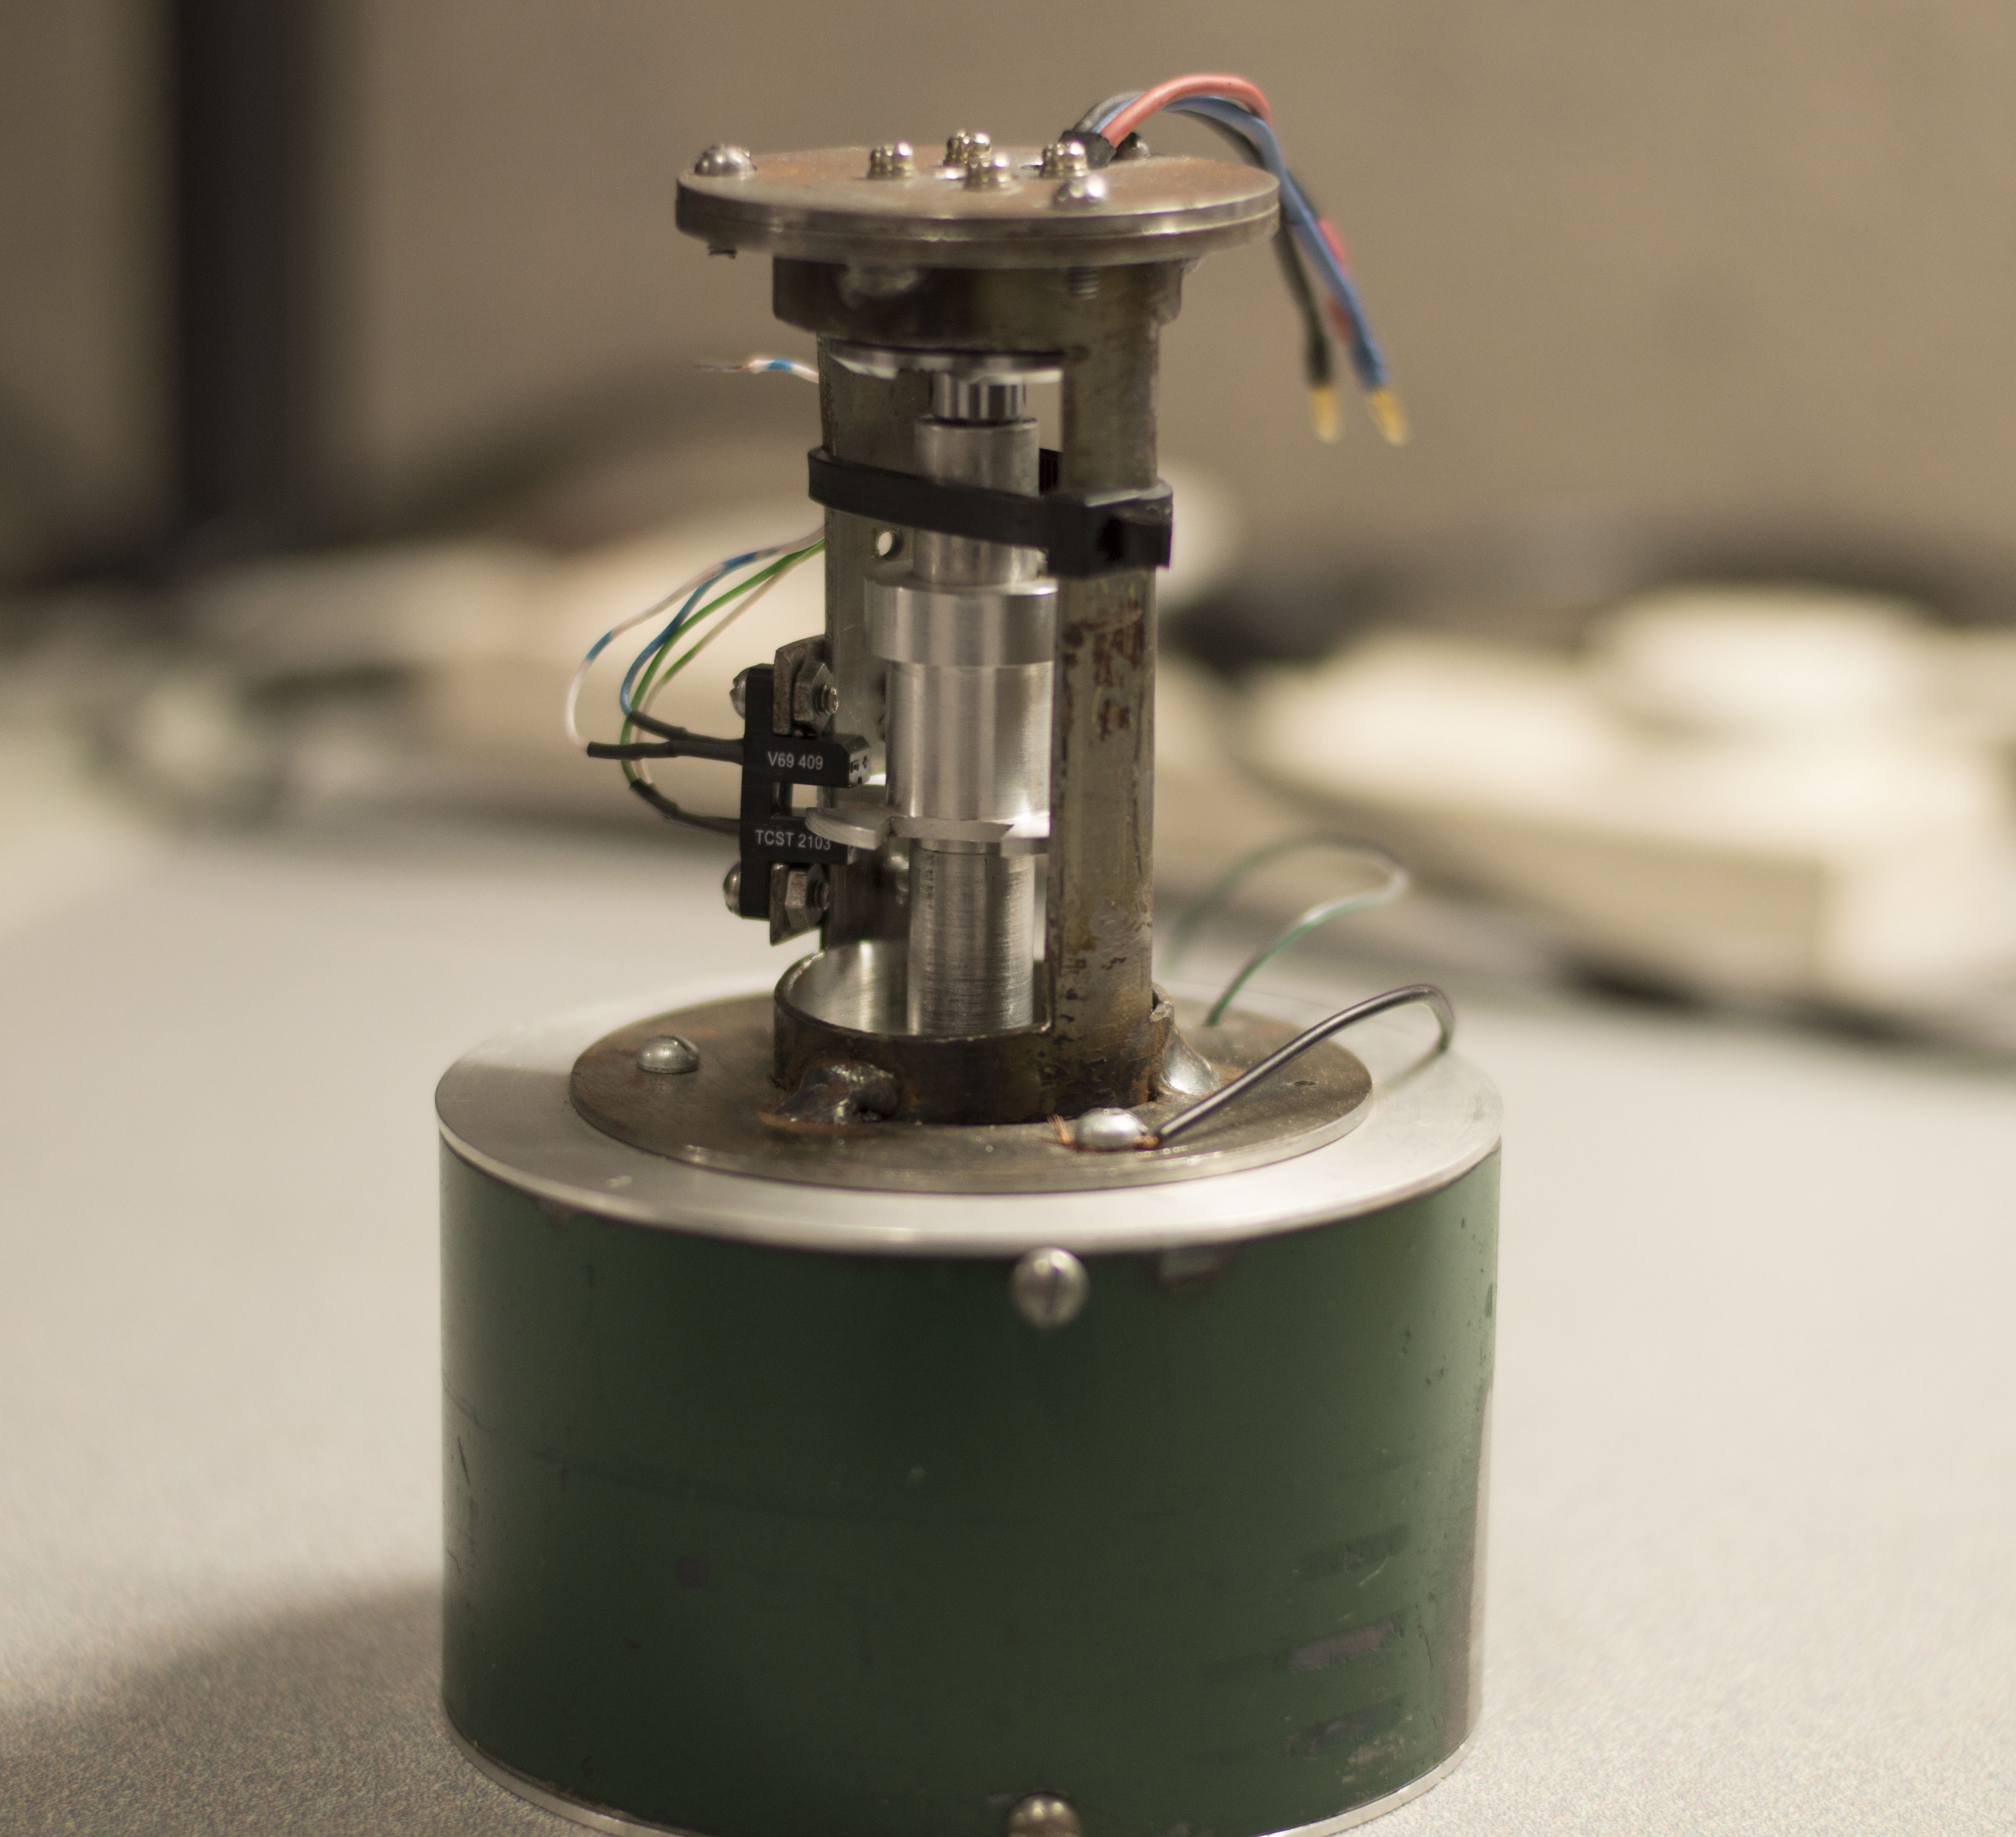
\includegraphics[width=0.80\textwidth, height = 7cm]{sensorvertical}
  \caption[Imagen del sensor de campo electrostatico utilizado (vertical)]{Foto del sensor en vertical. Puede verse en el eje, el sistema de aspas y fotointerruptor utilizado para medir las RPM.}\label{fig:sensorvertical}
\end{figure}

Ademas de las aspas que miden el campo electrico, en el eje del motor se encuentra un segundo grupo de aspas, pero mas pequeño; junto a estas aspas se encuentra acoplado un fotointerruptor, de manera que el paso de cada aspa interrumpe el paso de luz de un extremo a otro. Si se construye el circuito requerido para el fotointerruptor, ocurrira que cuando el motor este girando, se generen pulsos cuadrados a la salida del fotointerruptor, permitiendo obtener cuentas que ayudaran a la hora de controlar la velocidad del motor. Las aspas secundarias y el fotointerruptor pueden verse en la figura \ref{fig:sensorvertical}

% subsection el_sensor (end)

% section introduccion (end)

\section{Requerimientos de la iteracion} % (fold)
\label{sec:requerimientos_de_la_iteracion}

\begin{itemize}
\item Se deberian utilizar las funcionalidades de los sistemas desarrollados en el transcurso del proyecto para obtener mediciones del sensor
\item Se deberia controlar la velocidad del motor utilizando el fotointerruptor
\item Se deberia diseñar y construir una placa con un circuito de adaptacion para el funcionamiento y la operacion del sensor
\item La placa de adaptacion deberia poder ser acoplable a la placa de instrumentacion (como shield)
\item Se deberia construir un recipiente donde pueda entrar el sensor junto con el sistema de instrumentacion y el sistema gestionador, para poder colocarlo en el aire libre con el objetivo de realizar una prueba de campo
\end{itemize}


% section requerimientos_de_la_iteracion (end)

\section{Experimentacion} % (fold)
\label{sec:experimentacion}

El motor dentro de este sensor incluia un driver PWM. Para arrancar y dar velocidad a este motor, se utilizo, como primera instancia, una placa de desarrollo Arduino con un software hecho por Emiliano Pellicioni y Diego Gutierrez. Con el driver conectado a la placa y el programa funcionando, era posible arrancar el motor y darle una velocidad (aunque no muy constante).

Teniendo el motor funcionando, la teoria indica que el sensor esta midiendo campo. Para probar esto, se utilizo una regla de plastico cargada con electricidad estatica y un osciloscopio conectado a la salida del sensor. Al acercar y alejar la regla de las aspas, se podia ver en la salida del osciloscopio como la onda resultante a la salida del sensor aumentaba y disminuia en amplitud. Lo que estabamos viendo, en ese momento, era una salida ``en crudo'' del sensor. Para poder convertir la señal y obtener datos coherentes, era necesario rectificar la señal. \\

El fotointerruptor acoplado al eje del motor da la posibilidad de realizar un conteo de señales cuadradas que nos proporcione los datos suficientes como para realizar una medicion de las vueltas por minuto del motor. Necesita de un circuito basico para funcionar. Lo construimos en una protoboard junto con todo lo necesario para hacer funcionar el motor. Con ayuda de un osciloscopio, fue posible ver los pulsos cudadrados de 5 Volts generados por el fotointerruptor. Estos pulsos son los que luego servirian de entrada a un contador de eventos de la placa de instrumentacion, con el objetivo de controlar la velocidad del motor. \\

ACA FALTARIA INCLUIR IMAGENES DE:

-EL OSCILOSCOPIO CON LA SALIDA DEL SENSOR MIDIENDO
-EL OSCILOSCOPIO CON LA SALIDA DEL FOTO INTERRUPTOR

% section experimentacion (end)

\section{Adaptacion de la plataforma al sensor} % (fold)
\label{sec:adaptacion_de_la_plataforma_al_sensor}

\subsection{Circuito de adaptacion} % (fold)
\label{sub:circuito_de_adaptacion}

% subsection circuito_de_adaptacion (end)

Este sensor particular requiere de ciertos requerimientos para funcionar de manera correcta:

\begin{itemize}
  \item El motor deberia estar alimentado con una señal continua de 12 Voltios
  \item El driver del motor deberia estar conectado a una salida de un generador de señales moduladas en ancho de pulso, con un nivel de 5 Voltios en alto y 0 Voltios en bajo.
  \item La velocidad del motor deberia ser rapida y estable; priorizando la estabilidad a la velocidad.
  \item La señal de campo electrostatico deberia ser rectificada y amplificada previa a ser convertida a digital
\end{itemize}


Ademas de los requerimientos principales mencionados, fueron propuestos los siguientes requerimientos secundarios:

\begin{itemize}
  \item El diseño de la placa deberia ser tal que sea acoplable y desacoplable a la placa de instrumentacion.
  \item Deberia consumir lo menos posible
\end{itemize}

Para cumplir con estos requerimientos, fue necesario desarrollar funcionalidades aparte dentro del programa embebido en la plataforma de instrumentacion, ademas de un circuito de adaptacion acoplado a la misma.

% subsection requerimientos (end)
\subsubsection{Circuito de adaptacion para la señal de nivel de campo} % (fold)
\label{ssub:circuito_de_adaptacion_para_la_señal_de_nivel_de_campo}

La señal a la salida del sensor es alterna y de muy baja intensidad. El conversor analogico digital requiere de una señal rectificada y de un umbral minimo para funcionar correctamente. Para esto, se diseño un circuito de adaptacion de señal, que rectifica y amplifica la salida del sensor. Este circuito puede verse en la figura FIGURA.  

aca va el operacional con el amplificador y rectificador que se pone para que vaya antes del conversor.. con imagen



% subsection circuito_de_adaptacion_para_la_señal_de_nivel_de_campo (end)

\subsubsection{Circuito de adaptacion para la señal de pulsos del fotointerruptor} % (fold)
\label{ssub:circuito_de_adaptacion_para_la_señal_de_pulsos_del_fotointerruptor}


En esta configuracion, el fotointerruptor genera una señal de pulsos cuadrados a medida que el motor gira. Esta señal puede usarse como entrada a un contador de eventos, y de esta manera medir la velocidad de giro del motor. La figura \ref{fig:fotointerruptorcircuitotipico} muestra el circuito implementado para este fin. 

\begin{figure}[h]
  \centering
  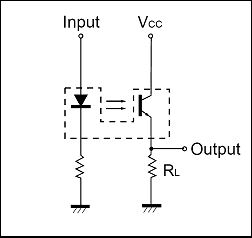
\includegraphics[width=0.80\textwidth, height = 7cm]{fotointerruptorcircuitotipico}
  \caption{Circuito utilizado para el fotointerruptor}\label{fig:fotointerruptorcircuitotipico}
\end{figure}

En esta disposicion, cuando el fotosensor esta iluminado, hay 5 Volts en la salida; de lo contrario 0 Volts. Esto hace que cuando el motor gira, las aspas van a tapar y destapar la entrada de luz al fotosensor generando una onda cuadrada a la salida del circuito, cuya frecuencia depende de la velocidad del motor. Dentro del software de la plataforma de instrumentacion, se utilizo uno de los contadores de eventos disponibles para obtener las cuetnas del fotoiterruptor y medir la velocidad del motor. Con esta informacion, se modifica el ancho de pulso de la señal PWM a la entrada del driver del motor. Corrigiendo asi la velocidad, para mantenerla lo mas estable posible. 

% subsection circuito_de_adaptacion_para_la_señal_de_pulsos_del_fotointerruptor (end)

\subsubsection{Circuito de alimentacion} % (fold)
\label{ssub:circuito_de_alimentacion}

La placa de instrumentacion esta diseñada para estar siempre encendida. Al no consumir mucho, no trae problemas de consumo o temperatura. Pero habiendo hecho esta adaptacion, era necesario tener en cuenta el consumo del motor mientras esta encendido pero sin girar. Para ahorrar consumo, propusimos agregar un control de encendido y apagado del sensor, utilizando uno de los pines GPIO del microcontrolador. \\

La figura PONER FIGURA DEL CIRCUITO muestra el circuito que prepara la señal del microcontrolador que controla el encendido y apagado del motor. Utilizamos un relé, un optoacoplador, un transistor, un diodo y resistencias. El optoacoplador sirve para aislar opticamente el circuito logico del motor con el circuito de 12 V. El rele electromecanico conmuta la conductividad entre el motor y masa, de manera que en un estado del rele el motor esta prendido, y en el otro esta apagado. Utilizamos un transistor porque los 5V a la salida del optoacoplador no eran suficientes para la tension de switching del relé.

% subsection circuito_de_alimentacion (end)

\subsubsection{Señal modulada en ancho de pulso para el adaptador del motor} % (fold)
\label{ssub:señal_modulada_en_ancho_de_pulso_para_el_adaptador_del_motor}

% aca en realidad no hicimos nada porque lo unico que hay es el cable de salida del pwm que viene de la placa y se conecta de pecho al driver.. pero bueno explicar eso.. y explicar tambnein que pasamos desde el arduino que hacia todo por interrupciones al pwm de la placa que lo hace todo por HW y funciona mucho mejor. aunque no explicar como funciona el programa porque eso va despues

El motor dentro de la estructura que conforma el motor tiene un modulo adaptador programable que funciona como interfaz, haciendo que una señal modulada en ancho de pulso se convierta en la velocidad de giro del motor, asi como tambien en distintas configuraciones. Los distintos anchos de pulso son codigos que representan distintos modos para el driver. En el manual, especifica las distintas configuraciones disponibles y como establecerlas utilizando distintas señales moduladas en ancho de pulso. Tanto en el proceso de configuracion como en el funcionamiento normal, el driver emite sonidos en distintos tonos que dan informacion sobre el estado en cada momento.

Para una respuesta estable del sensor, era importante que las aspas giren a una velocidad alta y constante. Alrededor de los 4000 RPM, priorizando la estabilidad a la velocidad. Dentro del programa de la plataforma de instrumentacion, existen rutinas que establecen el driver automaticamente en el modo requerido por nuestro sistema. Estas rutinas utilizan un modulo del microcontrolador denominado PCA, que incluye, en uno de sus modos, un generador de señal modulada en pulsos. Cuando el motor esta en funcionamiento, el mismo programa se encarga de estabilizar su velocidad con las funciones descritas en la seccion \ref{sec:software_de_adaptacion}


% subsection circuito_de_adaptacion_para_la_señal_modulada_en_ancho_de_pulso_para_el_driver_del_motor (end)

\subsubsection{Circuito final} % (fold)
\label{ssub:circuito_final}

En las secciones anteriores, describimos por separado cada una de las partes del circuito de adaptacion para el sensor de campo. La figura FIGURA muestra el despliegue de componentes del circuito final. Este diseño se imprimio en un PCB para acoplar a la plataforma de instrumentacion. El circuito impreso y acoplado se muestra en la figura FIGURA.


% subsection circuito_final (end)

% section implementacion_de_una_placa_de_adaptacion_para_el_sensor_de_campo (end)


\subsection{Software de adaptacion} % (fold)
\label{sec:software_de_adaptacion}


El circuito de adaptacion, prepara las señales de entrada y salida necesarias para el funcionamiento correcto del sensor. Dentro de la placa de instrumentacion, desarrollamos funcionalidades anexas al software principal para trabajar estas señales.
Realizamos un modulo aparte llamado ``sensor_CE'', cuyas funciones estan desarrolladas de manera especifica para este sensor. Estas funciones incluyen:

\begin{itemize}
	\item Dar arranque y parada al motor
	\item Controlar la velocidad del motor.
\end{itemize}

La medicion de campo no es parte del software de adaptacion, dado que se realiza utilizando funciones del modulo ``conversor''. La señal proveniente del circuito de adaptacion que corresponde a la telemetria proveniente del sensor, se conecta a uno de los pines de entrada del conversor analogico-digital. \\

La figura \ref{fig:diagramabloquessensor} muestra el diagrama de bloques de la adaptacion del software a la plataforma de instrumentacion.

\begin{figure}[h]
  \centering
  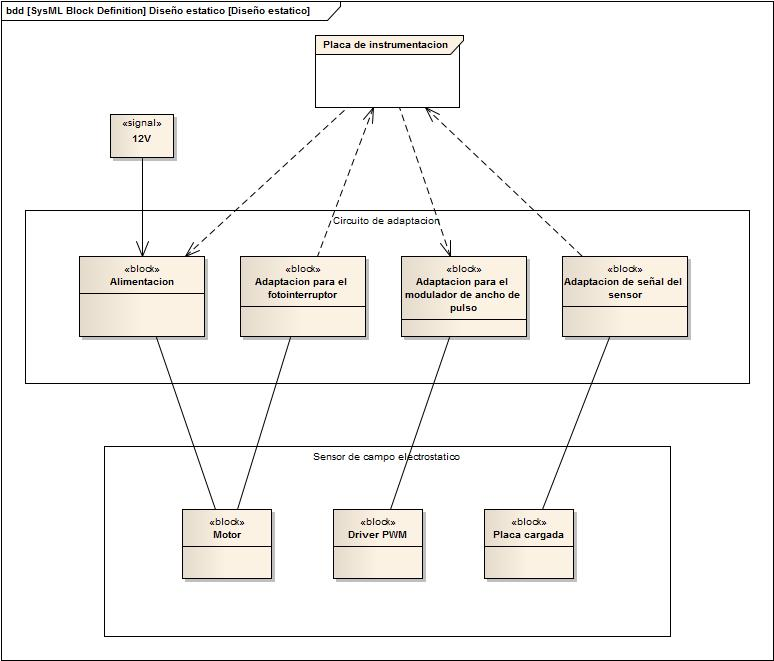
\includegraphics[width=0.80\textwidth, height = 7cm]{diagramabloquessensor}
  \caption{Diagrama de bloques fisicos del sistema de adaptacion del sensor}\label{fig:diagramabloquessensor}
\end{figure}

\subsubsection{Arranque y parada} % (fold)
\label{ssub:arranque_y_parada}

El motor esta controlado por un driver PWM que traduce señales moduladas en ancho de pulso en la corriente trifasica que da giro al motor. Para dar arranque al motor, es necesario seguir una serie de pasos que dependen del modo configurado en el driver. Para dar fin al giro del motor, simplemente hay que apagar la señal PWM. \\

Para este caso particular, es necesario utulizar un unico modo de configuracion, ya que se necesita que el motor gire a una unica velocidad, lo mas estable posible. El modo de configuracion esta establecido aunque el driver esta apagado. En caso de necesitar reconfigurarlo, existen funciones dentro del software de adaptacion que lo permiten. \\

Si el driver esta configurado correctamente y esta alimentado a 12 Voltios, es necesario activar la secuencia de arranque para que comience a girar. Esta secuencia de arranque consiste en 3 señales de distintos anchos de pulso separadas por intervalos de un segundo. Luego de esta secuencia, se establece el ancho de pulso que da la velocidad estable al motor, configurada en este caso para 4000 RPM. \\

Una vez que el motor alcanzo su velocidad estable, se activa el control de velocidad, para evitar que se desestabilice. 

% subsubsection arranque_y_parada (end)

\subsubsection{Control de velocidad} % (fold)
\label{ssub:control_de_velocidad}

La velocidad de giro del motor deberia ser rapida y constante para un mejor funcionamiento del motor, priorizando estabilidad a velocidad. Para lograr esto, utilizamos el fotointerruptor acoplado al sensor como generador de pulsos cuadrados. Estos pulsos se usan como entrada a uno de los contadores de eventos de la plataforma de instrumentacion. Con el valor de esta cuenta, es posible calcular la velocidad del motor en tiempo real, con una precision de unos 30 milisegundos por medicion. \\

La estabilidad en en la velocidad de giro del motor se alcanzo mediante un control basico de velocidad, hecho por software. Estableciendo una base de tiempo con uno de los timer del microcontrolador, se cuenta la cantidad de eventos sobre esa base de tiempo, la cantidad de cuentas entonces, da la velocidad. Una velocidad ``estable'' esta establecida en una variable fija, y se corresponde a una cantidad fija de eventos en la misma base de tiempo. Comparando la cantidad de eventos medidos sobre la base de tiempo con la cantidad de eventos que corresponden a la velocidad estable, se sabe si el motor esta girando demasiado rapido, o demasiado lento. Con esta informacion, se ajusta la velocidad del motor para acelerarlo o desacelerarlo, modificando el ancho de pulso del modulo PCA conectado al driver PWM del motor. Una descripcion grafica de este proceso se ilustra en la figura \ref{diagramaactividadescontrolvelocidad}

% subsubsection control_de_velocidad (end)

Y DE ACTIVIDAD PARA BER LA SUCESION DE COSAS QUE OCURREN CUANDO SE:
-PRENDE EL MOTOR
-SE CONTROLA VELOCIDAD

MAS QUE NADA.. ES LO MAS IMPORTANTE.

% section funcionalidades_desarrolladas_dentro_del_software_de_la_placa_de_instrumentacion_para_trabajar_junto_con_el_sensor (end)

\section{Pruebas} % (fold)
\label{sec:pruebas}

% section pruebas (end)

\section{Resultados} % (fold)
\label{sec:resultados}

% section resultados (end)

% chapter iteracion_7 (end)